%-------------------------------------------------------------------------------

% This file is part of Code_Saturne, a general-purpose CFD tool.
%
% Copyright (C) 1998-2016 EDF S.A.
%
% This program is free software; you can redistribute it and/or modify it under
% the terms of the GNU General Public License as published by the Free Software
% Foundation; either version 2 of the License, or (at your option) any later
% version.
%
% This program is distributed in the hope that it will be useful, but WITHOUT
% ANY WARRANTY; without even the implied warranty of MERCHANTABILITY or FITNESS
% FOR A PARTICULAR PURPOSE.  See the GNU General Public License for more
% details.
%
% You should have received a copy of the GNU General Public License along with
% this program; if not, write to the Free Software Foundation, Inc., 51 Franklin
% Street, Fifth Floor, Boston, MA 02110-1301, USA.

%-------------------------------------------------------------------------------

\programme{clptrg}


\vspace{1cm}
%%%%%%%%%%%%%%%%%%%%%%%%%%%%%%%%%%
%%%%%%%%%%%%%%%%%%%%%%%%%%%%%%%%%%
\section*{Function}
%%%%%%%%%%%%%%%%%%%%%%%%%%%%%%%%%%
%%%%%%%%%%%%%%%%%%%%%%%%%%%%%%%%%%
This subroutine is designed to realize the calculation of wall boundary conditions
for rough walls. The notations used are those introduced in \var{CONDLI} for general boundary
conditions.

The wall boundary conditions discussed herein are taken to include all the boundary conditions
for the velocity, the turbulent quantities ($k$, $\varepsilon$), the temperature when it has
a prescribed value at the wall (or the enthalpy and more generally
the {\it VarScalaires}\footnote{As in \fort{condli},{\it VarScalaire} will be used to designate
any variable, solution of a convection-diffusion equation, apart from the velocity, pressure and
the turbulent quantities $k$, $\varepsilon$.  The designation {\it VarScalaire} may be employed
particularly in relation to the temperature, the enthalpy or to a passive scalar.},
to be treated at the wall by applying a similarity law for the associated boundary layer.
For the {\it VarScalaires} especially, when the boundary conditions at the wall are
of the Neumann type (homogeneous or not), they are treated in \fort{condli} and hence will
not be discussed in this section. In particular, the boundary conditions of the  {\it VarScalaires}
representing the flux variance of other {\it VarScalaires} are not addressed here because
their treatment at the wall is of the homogeneous Neumann type.

We explain the method used to calculate the pair of coefficients $A_b$ and $B_b$, which are
used for the computation of certain discrete terms in the equations to solve and notably allow
us to determine a value associated to the boundary faces $f_{b,int}$ (at a point located
at the \begin{quotation}
centre
\end{quotation}of the boundary face, barycentre of its vertices) using the relation
$f_{b,int} = A_b+B_b\,f_{I'}$ ($f_{I'}$ is the value of the variable at point
$I'$, projection of the centre of the boundary cell on the normal to the boundary face
and passing through its centre: see figure~\ref{fig_flux_clptur}).

\begin{figure}[h]
\centerline{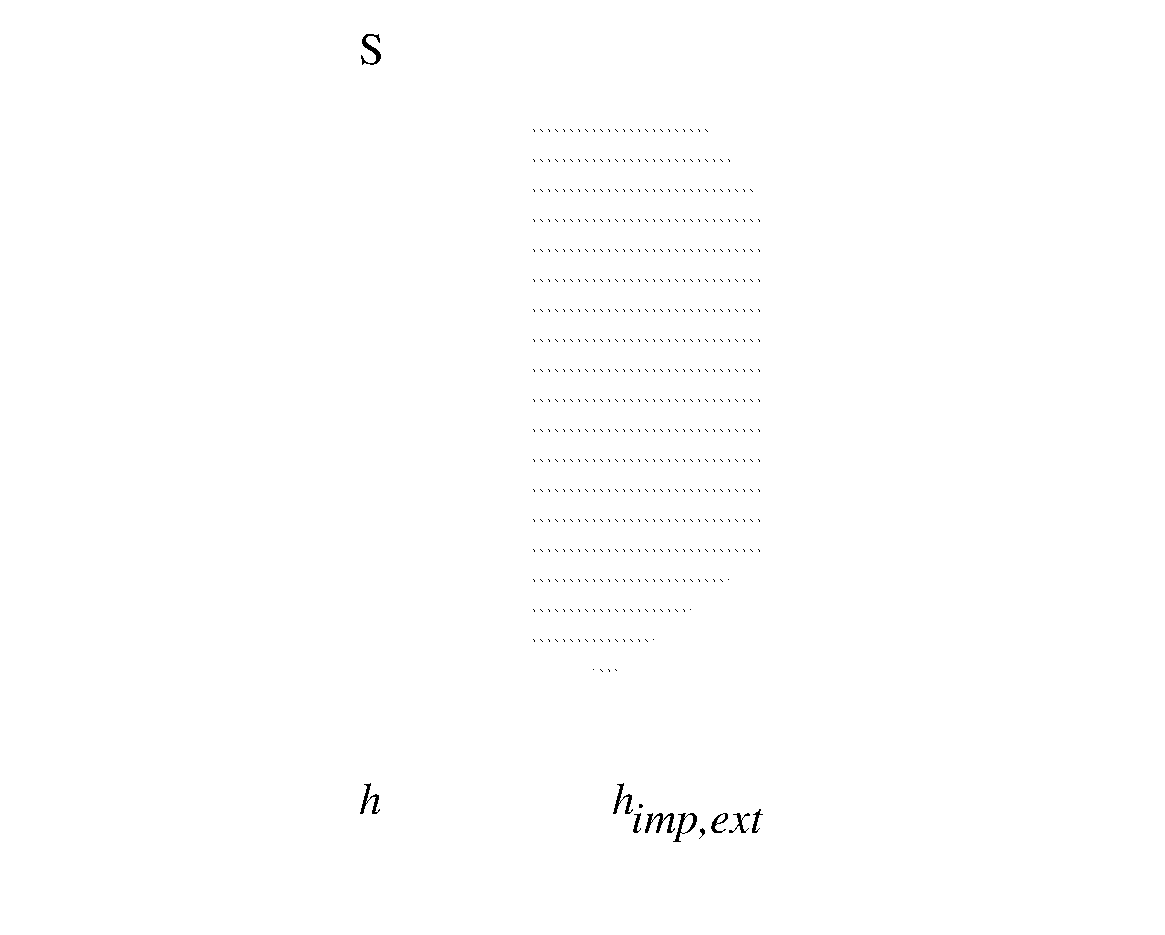
\includegraphics[height=7cm]{fluxbord}}
\caption{\label{fig_flux_clptur}Boundary cell.}
\end{figure}

%%%%%%%%%%%%%%%%%%%%%%%%%%%%%%%%%%
%%%%%%%%%%%%%%%%%%%%%%%%%%%%%%%%%%
\section*{Discretisation}
%%%%%%%%%%%%%%%%%%%%%%%%%%%%%%%%%%
%%%%%%%%%%%%%%%%%%%%%%%%%%%%%%%%%%

\etape{Notations\vspace{0,3cm}}
%%%%%%%%%%%%%%%%%%%%%%%%%%%%%%%%%%%%%%%%%%%%%%%%%%%%%%%%%%%%%%%%%%%%%%%%%%%%%%%
The velocity of the wall is noted $\vect{v}_p$ and is assumed to be projected onto
the plane tangent to the wall (if it is not, then it will be projected by the code).

The velocity of the fluid is noted by $\vect{u}$. An index, $I$, $I'$ or $F$, serves
to designate the point at which it is evaluated. The tangential velocity component in
relation to the wall is denoted $u_\tau$. The fluid velocity in the reference frame
attached to the wall (\begin{quotation}
relative
\end{quotation} velocity) is written $\vect{u}^r=\vect{u} - \vect{v}_p$.

The orthonormal coordinate system attached to the wall is written
$\hat {\mathcal R}=(\vect{\tau},\vect{\tilde{n}},\vect{b})$.
\begin{itemize}
\item [$\bullet$] $\vect{\tilde{n}}=-\vect{n}$ is the unit vector orthogonal to the wall
and directed towards the interior of the computational domain.
\item [$\bullet$] $\vect{\tau} = \displaystyle\frac{1}{\|\vect{u}^r_{I'}-(\vect{u}^r_{I'}\,.\,\vect{\tilde{n}})\|}\left[\vect{u}^r_{I'}-(\vect{u}^r_{I'}\,.\,\vect{\tilde{n}})\right]$ is the unit vector parallel to the projection of the relative velocity at $I'$, $\vect{u}^r_{I'}$,
in the plane tangent to the wall ({\it i.e.} orthogonal to $\vect{\tilde{n}}$): see
figure~\ref{fig_flux_clptur}.
\item [$\bullet$] $\vect{b}$ is the unit vector completing the direct coordinate system.
\end{itemize}

\vspace{0.5cm}

In the {\bf two velocity scale model}, we employ the following notations:
\begin{itemize}
\item [-] $u_k$ the friction velocity at the wall obtained from the turbulent kinetic energy.

\item [-] $u^*$ the wall friction velocity calculated using the relationship given by $ \displaystyle\frac{u^r_{\tau,I'}}{u^*} = f(z_p)$.

\item [-] $z_p$  represents a dimensionless wall distance
      (this being the distance from the edge of the computational domain), namely
$z_p= I'F$ (see figure~\ref{fig_flux_clptur}). The function $f$ expresses the ideal form of
the velocity profile. In air, this function is given by a logarithmic law that takes account of
the dynamic surface roughness of the wall $z_0$:

$f(z_p)= \displaystyle\frac{1}{\kappa} ln \left ( \displaystyle \frac
      {z_p+z_0}{z_0} \right ) $

\item [-] The velocity scales, $u_k$ and $u^*$, are easy to compute, although their
computation does require knowledge of the turbulent energy $k_I$ at the centre of the
adjoining cell to the boundary face.

\item [-] The two-scale model is set as the default model in \CS. It
frequently enables minimizing, particularly in cases with heat transfer, the effects
of certain deficiencies in the $k-\varepsilon$ model (the impacting jet being
a classic example).
\end{itemize}

We will use $u^*$ and $u_k$ later, for the boundary conditions pertaining to the velocity
and the scalars (notably, the temperature).


\begin{equation}
\label{Eq_Mod_'2ech_Vit}
\begin{array}{l}
\text{\bf Two-velocity-scale model}\\
\left\{\begin{array}{l}
u_k = C_\mu^\frac{1}{4}k_I^\frac{1}{2}\\
u^* \text{solution of }  \displaystyle\frac{u^r_{\tau,I'}}{u^*} =
\displaystyle\frac{1}{\kappa}ln(z_k)\\
z_k=\displaystyle\frac{I'F+z_0}{z_0} = \displaystyle\frac{z_p+z_0}{z_0}\\
\text{   with   } C_\mu =0.09 \text{  and }  \kappa = 0.42
\end{array}\right.\\
\end{array}
\end{equation}


\vspace{0.5cm}

In the case of the one velocity scale model, $u^*$ denotes the only friction velocity
at the wall, obtained by solving the equation $\displaystyle\frac{u^r_{\tau,I'}}{u^*} = f(z_p)$.
The quantity $z_p$  represents a dimensionless wall distance, given by $z_p=I'F$. The
function $f$ reflects the ideal form of the velocity profile as in the case of the two
velocity scale model. Note that this friction velocity, the calculation of which is more
complicated (fixed point), can nevertheless be obtained without reference to the turbulent
variables ($k$, $\varepsilon$). For convenience, in the one-scale model we write $u_k=u^*$ .

We will use $u^*$ and $u_k$ later, for the boundary conditions pertaining to the velocity
and the scalars (notably, the temperature).

\begin{equation}
\begin{array}{l}
\text{\bf One velocity scale model}\\
\left\{\begin{array}{l}
u_k = u^*\\
u^* \text{solution of }  \displaystyle\frac{u^r_{\tau,I'}}{u^*} =
\displaystyle\frac{1}{\kappa}ln(z_k)\\
z_k=\displaystyle\frac{I'F+z_0}{z_0} = \displaystyle\frac{z_p+z_0}{z_0}\\
\text{   with   } C_\mu =0.09 \text{  and }  \kappa = 0.42
\end{array}\right.\\
\end{array}
\end{equation}

\etape{Boundary conditions for the velocity in $k-\varepsilon$\vspace{0,3cm}}
%%%%%%%%%%%%%%%%%%%%%%%%%%%%%%%%%%%%%%%%%%%%%%%%%%%%%%%%%%%%%%%%%%%%%%%%%%%%%%%
We first consider the conditions used in calculations performed with the
$k-\varepsilon$ model, as these are the most complex and the more general cases.

The boundary conditions are necessary in order to impose sufficient tangential
stress $\sigma_\tau=\rho_Iu^*u_k$ at the boundary in the momentum
equation\footnote{Proposition de modification des conditions aux limites de
paroi turbulente pour le Solveur Commun dans le cadre du mod\`ele
$k-\varepsilon$ standard ({\it \begin{quotation}
Proposed modification of the turbulent wall boundary conditions for the
Common Solver in the frame of the standard $k-\varepsilon$ model
\end{quotation} }), EDF report HI-81/00/019/A, 2000, M. Boucker, J.-D. Mattei.}
($\rho_I$ is the density at the centre of cell $I$). The term requiring the boundary
conditions is the one that contains the normal derivative of the velocity at the wall,
this being\footnote{The transpose gradient term is dealt with in \fort{visecv}
and will not be considered here.}: $(\mu_I+\mu_{t,I})\ggrad{\vect{u}}\,\vect{n}$.
It appears in the second member of the usual
momentum equation (see \fort{bilsc2} and \fort{predvv}).

When the $k-\varepsilon$ model shows a tendency to overestimate the turbulent kinetic
energy production, the length scale of the model, $L_{k-\varepsilon}$, can become
significantly larger than the maximum theoretical scale of turbulent boundary layer
eddies $L_{\text{theo}}$. We write:
\begin{equation}
\left\{\begin{array}{l}
L_{k-\varepsilon} = C_{\mu}\displaystyle\frac{k^\frac{3}{2}}{\varepsilon}\\
L_{\text{theo}} = \kappa\, \left( I'F+z_0 \right) = \kappa\, \left(z_p+z_0 \right)
\end{array}\right.
\end{equation}

If $L_{k-\varepsilon}>L_{\text{theo}}$, we then have  $\mu_{t,I}>\mu_{t}^{lm}$
with $\mu_{t,I}$ the turbulent viscosity of the $k-\varepsilon$ model at
point $I$ and $\mu_{t}^{lm}=\rho_I L_{\text{theo}}u_k$ the turbulent
viscosity of the mixing length model. Moreover, the tangential stress
can be written with the turbulent viscosity being made to appear:
\begin{equation}
\sigma_\tau = \rho_Iu^*u_k = \displaystyle\frac{u^*}{\kappa\,
 \left(I'F+z_0 \right)}
\underbrace{\rho_I\kappa\, \left( I'F+z_0 \right)  u_k}_{\mu^{lm}_t}
\end{equation}
The viscosity scale introduced in this expression of the stress is thus at odds
with the one derived from the turbulence computed locally by the model. We therefore
prefer to write the stress so that the $k-\varepsilon$ length scale is used whenever
it is lower than the limit $L_{\text{theo}}$:
\begin{equation}
\sigma_\tau = \displaystyle\frac{u^*}{\kappa\, \left(I'F+z_0 \right)} max(\mu_{t}^{lm},\mu_{t,I})
\end{equation}

This value can then be used for the diffusive flux calculation which is dependent on the
stress in the Navier-Stokes equation:
\begin{equation}\label{eq_grad_sigma_clptur}
(\mu_I+\mu_{t,I})\ggrad{\vect{u}}\,\vect{n}=-\sigma_\tau \vect{\tau}
\end{equation}

However, the velocity gradient (gradient at the boundary face) is computed by the
code in the following form:
\begin{equation}\label{eq_grad_uf_clptur}
(\mu_I+\mu_{t,I})\ggrad{\vect{u}}\,\vect{n}=
\displaystyle\frac{(\mu_I+\mu_{t,I})}{\overline{I'F}}(\vect{u}_F-\vect{u}_{I'})
\end{equation}

Drawing on the approximate relationship between (\ref{eq_grad_sigma_clptur}) and
(\ref{eq_grad_uf_clptur}), we derive the value of $\vect{u}_F$ to impose,
denoted $\vect{u}_{F,flux}$~(conservation of the momentum flux):
\begin{equation}\label{eq_uf_flux_clptur}
\begin{array}{ll}
\vect{u}_{F,flux}&=\vect{u}_{I'}-\displaystyle\frac{\overline{I'F}}{\mu_I+\mu_{t,I}}\sigma_\tau \vect{\tau}\\
                 &=\vect{u}_{I'}-\displaystyle\frac{u^*}{\kappa\,
		  (\mu_I+\mu_{t,I})} max(\mu_{t}^{lm},\mu_{t,I})
		  \, \displaystyle\frac {I'F} {\left(I'F+z_0 \right)} \vect{\tau}
\end{array}
\end{equation}

In actual fact, a further approximation is made. This consists in imposing
zero normal velocity at the wall and using the equation (\ref{eq_uf_flux_clptur})
projected onto the plane tangent to the wall:
\begin{equation}
\vect{u}_{F,flux}=\left[u_{\tau,I'}-\displaystyle\frac{u^*}{\kappa\,
(\mu_I+\mu_{t,I})} max(\mu_{t}^{lm},\mu_{t,I}) \, \displaystyle\frac {I'F} {\left(I'F+z_0 \right)} \right]\vect{\tau}
\end{equation}

Lastly, it is also possible to make the wall velocity appear in the final expression:
\begin{equation}
\begin{array}{l}
\text{\bf Flux-type boundary conditions on the velocity}\,(k-\varepsilon)\\
\left\{\begin{array}{l}
\vect{u}_{F,flux}=\vect{v}_p+\left[u^r_{\tau,I'}-\displaystyle\frac{u^*}{\kappa\,
(\mu_I+\mu_{t,I})} max(\mu_{t}^{lm},\mu_{t,I})  \, \displaystyle\frac {I'F} {\left(I'F+z_0 \right)}\right]\vect{\tau}
\end{array}\right.\\
\end{array}
\end{equation}

A first pair of coefficients $A_{flux}$ and $B_{flux}$ is thence inferred (separately
for each velocity component) and is only used in the calculation of the tangential
stress dependent term (see \fort{bilsc2}):
\begin{equation}
\begin{array}{l}
\text{\bf Coefficients associated with the flux-type boundary conditions on the
velocity} (k-\varepsilon)\\
\left\{\begin{array}{l}
\vect{A}_{flux}=\vect{v}_p+\left[u^r_{\tau,I'}-\displaystyle\frac{u^*}{\kappa\,
(\mu_I+\mu_{t,I})} max(\mu_{t}^{lm},\mu_{t,I}) \, \displaystyle\frac {I'F} {\left(I'F+z_0 \right)} \right]\vect{\tau} \\
\vect{B}_{flux} = \vect{0}
\end{array}\right.
\end{array}
\end{equation}

Having seen above how to impose a boundary condition so as to correctly calculate the stress term,
we now need to take a closer look at the calculation of velocity gradients. We are seeking a
boundary face value which will allow us to obtain, with the formulation adopted for the gradient,
a value of turbulent production as close as possible to the theoretical value (determined using the
logarithmic law), in order to evaluate the normal derivative of the tangential velocity.
Hence, we define (at point $I$):
\begin{equation}\label{eq_ptheo_clptur}
P_{\text{theo}} = \rho_I u^* u_k
\|\displaystyle\frac{\partial u_\tau}{\partial\vect{n}}\|_{I} =
\rho_I \displaystyle\frac{u_k(u^*)^2}{\kappa\, \left(I'F+z_0 \right)}
\end{equation}

Moreover, the dominant term of the production computed in cell $I$ for typical situations (where $z$ is the coordinate on the $\vect{\tilde{n}}$ direction vector axis) is:
\begin{equation}
P_{\text{calc}} =
\mu_{t,I}\left(\displaystyle\frac{\partial u_\tau}{\partial z}\right)^2_{I}
\end{equation}

\begin{figure}[h]
\centerline{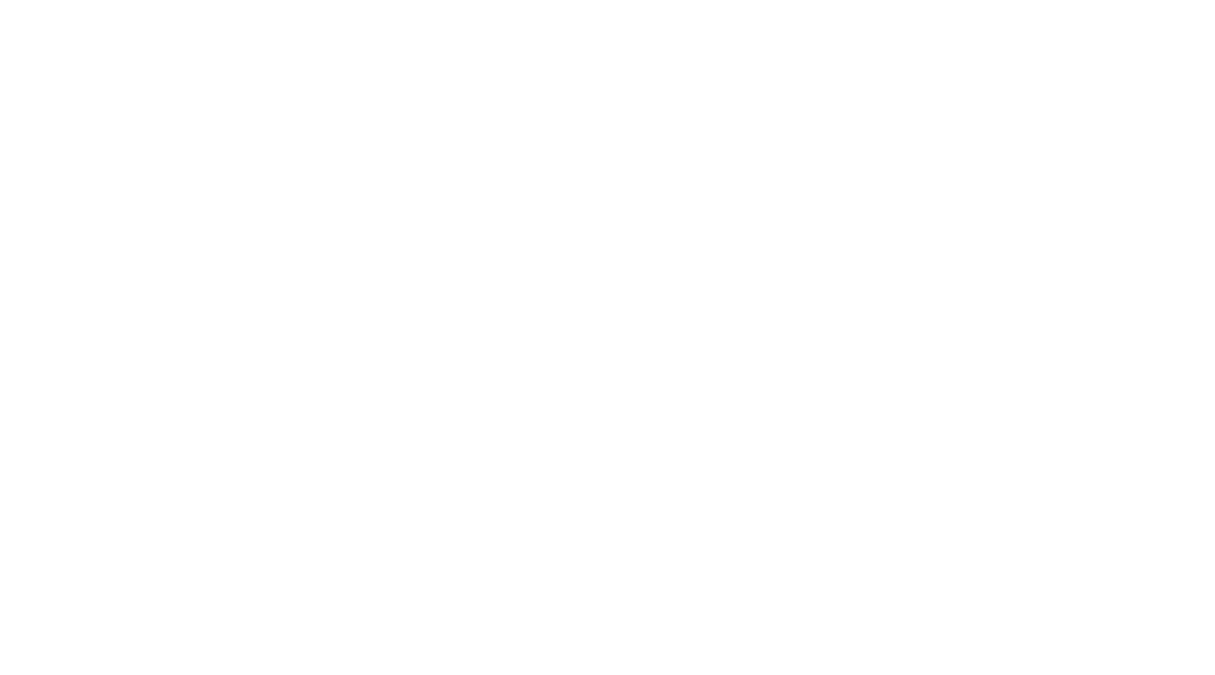
\includegraphics[height=7cm]{bordortho}}
\caption{\label{fig_bord_ortho_clptur}Boundary cell - Orthogonal mesh.}
\end{figure}

The normal gradient of the tangential velocity (cell gradient) is calculated in the code
using finite volumes and takes the following expression on regular orthogonal mesh (see the notations on figure~\ref{fig_bord_ortho_clptur}):
\begin{equation}
P_{\text{calc}} =
\mu_{t,I}\left(\displaystyle\frac{u_{\tau,G}-u_{\tau,F}}{2d}\right)^2 =
\mu_{t,I}\left(\displaystyle\frac{u_{\tau,I}+u_{\tau,J}-2u_{\tau,F}}{4d}\right)^2
\end{equation}
We then assume that $u_{\tau,J}$ can be obtained from $u_{\tau,I}$
and the normal gradient of $u_{\tau}$ evaluated at G based on the logarithmic
law, such that:
\begin{equation}
\label{eq_dvp_lim_utau}
u_{\tau,J}=u_{\tau,I}+ IJ\,.\,(\partial_z u_{\tau})_G+\mathcal{O} (IJ^{\,2}) \approx
u_{\tau,I}+ IJ\,.\,\left[\partial_z \left(\displaystyle
\frac{u^*}{\kappa}\,ln{ (z)} \right)\right]_G=
u_{\tau,I}+2d \, \displaystyle\frac{u^*}{\kappa \left(2d + z_0\right)}
\end{equation}
from which we obtain:
\begin{equation}\label{eq_pcalc_clptur}
\begin{array}{lll}
P_{\text{calc}}
&=&\mu_{t,I}\left(\displaystyle\frac{2u_{\tau,I}+2d  \, \displaystyle\frac{\,u^*}{\kappa
	     \left(2d + z_0\right) } -2u_{\tau,F}}{4d}\right)^2 \\
&=&
\mu_{t,I}\left(\displaystyle\frac{u_{\tau,I}+d \,\displaystyle\frac{\,u^*}{\kappa
	  \left(2d + z_0\right)} -u_{\tau,F}}{2d}\right)^2
\end{array}
\end{equation}

We then link equations (\ref{eq_ptheo_clptur}) and (\ref{eq_pcalc_clptur}) in order to impose
the equality of the production calculated and the theoretical turbulent production.
Application of the above formulae is extended without caution to non-orthogonal meshes
(the velocity at $I$ is simply evaluated at $I'$). The following expression is
then obtained for $u_{\tau,F}$:
\begin{equation}
u_{\tau,F,grad} =u_{\tau,I'}-\displaystyle\frac{u^*}{\kappa}\left(
2d\sqrt{\displaystyle\frac{\rho_I\kappa\, u_k }{\mu_{t,I} \left(I'F
							   +z_0\right) }
}-\displaystyle\frac{1}{2 + z_0/I'F}\right)
\end{equation}

A limit is then set on the gradient so that it remains at least as steep as the
gradient obtained from the normal derivative of the theoretical (logarithmic) velocity
profile at $I'$:\\
$\partial_z u_{\tau} = \partial_z (\displaystyle
\frac{u^*}{\kappa}\,ln{ (z)} ) =\displaystyle\frac{u^*}{\kappa\,\left(I'F + z_0\right) }$, thus
yielding:
\begin{equation}
u_{\tau,F,grad} =u_{\tau,I'}-\displaystyle\frac{u^*}{\kappa}max\left(1,
2d\sqrt{\displaystyle\frac{\rho_I\kappa\, u_k }{\mu_{t,I} \left(I'F + z_0\right)}}-\displaystyle\frac{1}{2 + z_0/I'F}\right)
\end{equation}


A condition of zero normal velocity at the wall is imposed.
Moreover, if the tangential velocity at $I'$ is zero
(absolute value below an arbitrary numerical limit of
$10^{-12}$), a no-slip condition is applied. We can then
also make the velocity of the wall appear in the final expression:
\begin{equation}
\begin{array}{l}
\text{\bf Gradient boundary conditions on the velocity} (k-\varepsilon)\\
\left\{\begin{array}{l}
\vect{u}_{F,grad}=\vect{v}_p
          \qquad\qquad\text{ if } u^r_{\tau,I'} < 10^{-12}  \\
\vect{u}_{F,grad}=\vect{v}_p +
u^r_{\tau,I'}-\displaystyle\frac{u^*}{\kappa}\left[max\left(1,2d\sqrt{\displaystyle\frac{\rho_I\kappa\, u_k }{\mu_{t,I}
\left(I'F + z_0\right)}}-\displaystyle\frac{1}{2 + z_0/I'F}\right)\right] \vect{\tau}
\end{array}\right.
\end{array}
\end{equation}

A second pair of coefficients, $A_{grad}$ and $B_{grad}$, is thereby inferred (separately
for each velocity component) and is used (with the exception of the terms depending on the
tangential stress, these being treated in \fort{bilsc2} using the coefficients $A_{flux}$
and $B_{flux}$)whenever the velocity gradient is required:
\begin{equation}
\begin{array}{l}
\text{\bf Coefficients associated with the gradient-type boundary conditions on the velocity }\\
\qquad\qquad\qquad\qquad\text{\bf} (k-\varepsilon)\\
\left\{\begin{array}{l}
\vect{A}_{grad}=\vect{v}_p
                    \qquad\qquad\text{ \ si\ } u^r_{\tau,I'} < 10^{-12}  \\
\vect{A}_{grad}=\vect{v}_p+
 u^r_{\tau,I'}-\displaystyle\frac{u^*}{\kappa}\left[max\left(1,2d\sqrt{\displaystyle\frac{\rho_I\kappa\, u_k }{\mu_{t,I}
\left(I'F + z_0\right)}}-\displaystyle\frac{1}{2 + z_0/I'F}\right)\right] \vect{\tau}\\
\vect{B}_{grad} = \vect{0}
\end{array}\right.
\end{array}
\end{equation}

\newpage

\etape{Boundary conditions for the $k$ and $\varepsilon$ variables (standard
$k-\varepsilon$ model)\vspace{0,3cm}}

We impose a Dirichlet condition derived from the friction velocity
$u_k$ (refer to equation~(\ref{Eq_Mod_'2ech_Vit})) on $k$:
\begin{equation}
k= \displaystyle\frac{u_k^2}{C_\mu^\frac{1}{2}}
\end{equation}


We want to set the normal derivative of $\varepsilon$ based on the following
theoretic law  (refer to the notations in figure \ref{fig_bord_ortho_clptur}):
\begin{equation}\label{eq_partialep_theo_clptur}
G_{\text{theo},\varepsilon} = \displaystyle\frac{\partial}{\partial z}
 \left[ \displaystyle\frac{u_k^3}{\kappa\, \left(z + z_0\right)}\right]
\end{equation}



The point $M$ is used to impose a boundary condition with a higher order accuracy
in space. In effect, using the simple relation
$\varepsilon_F=\varepsilon_I+d\partial_z\varepsilon_I + O(d^2)$ leads to an
accuracy of order 1.
Second-order accuracy can be obtained using the following truncated series expansions:
\begin{equation}
\left\{\begin{array}{ll}
\varepsilon_M&=\varepsilon_I-\displaystyle\frac{d}{2}\partial_z\varepsilon_I+\displaystyle\frac{d^2}{8}\partial^2_z\varepsilon_I+O(d^3)\\
\varepsilon_M&=\varepsilon_F+\displaystyle\frac{d}{2}\partial_z\varepsilon_F+\displaystyle\frac{d^2}{8}\partial^2_z\varepsilon_F+O(d^3)
\end{array}\right.
\end{equation}
The difference between the above two expansions, can be expressed as
\begin{equation}\label{eq_epsf_clptur}
\varepsilon_F=\varepsilon_I-\displaystyle\frac{d}{2}(\partial_z\varepsilon_I+\partial_z\varepsilon_F)+O(d^3)
\end{equation}
Moreover, we have
\begin{equation}
\left\{\begin{array}{ll}
\partial_z\varepsilon_I&=\partial_z\varepsilon_M+d\partial^2_z\varepsilon_M+O(d^2)\\
\partial_z\varepsilon_F&=\partial_z\varepsilon_M-d\partial^2_z\varepsilon_M+O(d^2)
\end{array}\right.
\end{equation}
The sum of the latter two expansions enables us to establish that
$\partial_z\varepsilon_I+\partial_z\varepsilon_F=2\partial_z\varepsilon_M+O(d^2)$ which, when
substituted back into (\ref{eq_epsf_clptur}), provides the desired second-order accurate
approximation of $\varepsilon_F$:
\begin{equation}
\varepsilon_F=\varepsilon_I-d\partial_z\varepsilon_M+O(d^3)
\end{equation}
The term $\partial_z\varepsilon_M$ is evaluated against the theoretical value (\ref{eq_partialep_theo_clptur})
and the value to impose at the boundary ($d=I'F$) thence obtained:
\begin{equation}
\varepsilon_F=\varepsilon_I+d\displaystyle\frac{ u_k^3}{\kappa\, (d/2+ z_0)^2}
\end{equation}


This relation is extended without caution for application on non-orthogonal meshes
(which is bound to degrade the order of accuracy in space).

We finally obtain the:

\begin{equation}
\begin{array}{l}
\text{\bf Boundary conditions on } k \text { \bf and } \varepsilon \\
\left\{\begin{array}{ll}
k_F&= \displaystyle\frac{u_k^2}{C_\mu^\frac{1}{2}}\\
\varepsilon_F&=\varepsilon_{I'}+I'F\displaystyle\frac{ u_k^3}{\kappa\,
 (I'F/2 + z_0)^2}
\end{array}\right. \\
\end{array}
\end{equation}
and the associated coefficients
\begin{equation}
\begin{array}{l}
\text{\bf Coefficients associated with the boundary conditions on the variables }
k \text { \bf and } \varepsilon \\
\left\{\begin{array}{llll}
A_k&= \displaystyle\frac{u_k^2}{C_\mu^\frac{1}{2}} &\text{ et } B_k&= 0 \\
A_\varepsilon&=I'F\displaystyle\frac{ u_k^3}{\kappa\, (I'F/2 + z_0)^2}&\text{ et } B_\varepsilon&= 1
\end{array}\right.\\
\end{array}
\end{equation}

\newpage
\etape{Boundary conditions for the {\it VarScalaires}\vspace{0,3cm}}
Only the boundary conditions with a prescribed value (at the wall or in the near-wall
region with, eventually, an external transfer coefficient) are addressed herein. We
draw on the notations taken from figure \ref{fig_flux_clptur} and the general presentation
provided in \fort{condli}, the essential elements of which are resumed below.

The conservative form of the normal flux at the boundary for the variable $f$ is written:
\begin{equation}\label{eq_flux_clptur}
\begin{array}{l}
    \underbrace{h_{int}(f_{b,int}-f_{I'})}_{\phi_{int}}
  = \underbrace{h_{b}(f_{b,ext}-f_{I'})}_{\phi_{b}}
  = \left\{\begin{array}{ll}
    \underbrace{h_{imp,ext}(f_{imp,ext}-f_{b,ext})}_{\phi_{\text{\it imposed real}}} &\text{(Dirichlet condition)}\\
    \underbrace{\phi_{\text{\it imp,ext}}}_{\phi_{\text{\it imposed real}}}
            &\text{(Neumann condition)}
           \end{array}\right.
\end{array}
\end{equation}


These two equations are rearranged in order to obtain the numerical flux value
$f_{b,int}=f_{F}$ to impose at the wall surface, given the values of
$f_{imp,ext}$ and $h_{imp,ext}$ set by the user and the value of $h_{b}$
determined according to the laws of similarity detailed hereafter. Coefficients $A$
and $B$, are derived directly from the boundary condition, as specified below.

\begin{equation}\label{eq_fbint_clptur}
\begin{array}{l}
\text{\bf Boundary conditions on the {\it VarScalaires} }\\
f_{b,int} =
\underbrace{\displaystyle\frac{h_{imp,ext}}{h_{int}+h_r h_{imp,ext} } f_{imp,ext}}_{A} +
\underbrace{\displaystyle\frac{h_{int}+h_{imp,ext}(h_r-1)}{h_{int}+h_r h_{imp,ext} }}_{B} f_{I'}
\text{  with } h_r=\displaystyle\frac{h_{int}}{h_{b}}
\end{array}
\end{equation}


\newpage
{\bf Principle of similarity: calculation of } $h_b$.

The only remaining unknown in the expression (\ref{eq_fbint_clptur}) is $h_{b}$, with $h_{int}$
being a numerical value consistent with the calculation method used to compute the face
gradients and specified in \fort{condli} ($h_{int}=\displaystyle\frac{\alpha}{\overline{I'F}}$). The
value of $h_{b}$ must relate the flux to the difference between the values of $f_{I'}$ and $f_{b,ext}$
taking the boundary layer into account (the profile of $f$ is not always linear):
\begin{equation}
\phi_b=h_b\,(f_{b,ext}-f_{I'})
\end{equation}

The theoretical considerations and their application are presented below, using the general
notations. In particular, the Prandtl-Schmidt number is noted
$\sigma=\displaystyle\frac{\nu\,\rho\,C}{\alpha}$.
When the scalar $f$ under consideration is the temperature,
we have (see \fort{condli}):
\begin{list}{$\bullet$}{}
\item $C=C_p$ (specific heat capacity),
\item $\alpha=\lambda$ (molecular conductivity),
\item $\sigma = \displaystyle\frac{\nu\,\rho\,C_p}{\lambda} = Pr$
       (Prandtl number),
\item $\sigma_t = Pr_t$ (turbulent Prandtl number),
\item $\phi=\left(\lambda+\displaystyle\frac{C_p\mu_t}{\sigma_t}\right)
        \displaystyle\frac{\partial T}{\partial z}$ (flux in $Wm^{-2}$).
\end{list}

J. R. Garratt's "The atmospheric boundary layer", Cambridge University Press was used
as a supporting reference.

The flux at the wall for the scalar $f$ is written:
\begin{equation}\label{Eq_Flux_scalaire}
\phi = -\left(\alpha+C\,\frac{\mu_t}{\sigma_t}\right)
                  \frac{\partial f}{\partial z}
     = -\rho\,C \left(\displaystyle\frac{\alpha}{\rho\,C}+
                                \frac{\mu_t}{\rho\sigma_t}\right)
                  \frac{\partial f}{\partial z}
\end{equation}

(the flux is positive if it is directed into the fluid domain, as indicated
by the orientation of the $z$ axis).

\noindent Similarly for the temperature, with $a=\displaystyle\frac{\lambda}{\rho\,C_p}$ and
$a_t=\displaystyle\frac{\mu_t}{\rho\,\sigma_t}$, we have:
\begin{equation}
\phi = -\rho\,C_p(a+a_t)\frac{\partial T}{\partial z}
\end{equation}

\noindent We introduce $f^*$ in order to make $f$ dimensionless, using the boundary flux
value $\phi_b$:
\begin{equation}
f^* = -\displaystyle\frac{\phi_b}{\rho\,C\,u_k}
\end{equation}
For the temperature, this yields:
\begin{equation}
T^* = -\displaystyle\frac{\phi_b}{\rho\,C_p\,u_k}
\end{equation}

\noindent As was noted beforehand, in the two-velocity scale model, $u_k$ is the
wall friction velocity obtained from the mean kinetic energy of the turbulent
motion\footnote{$u_k = C_\mu^\frac{1}{4}k_I^\frac{1}{2}$}. For the
one velocity scale model, we set $u_k=u^*$ with $u^*$ the wall friction velocity
determined from the logarithmic law.

We then divide both sides of equation~(\ref{Eq_Flux_scalaire})
by $\phi_b$. Given that the flux is conserved, $\phi=\phi_b$ so the left side of
the equation is simplified to 1. On the right-hand side, we replace
$\phi_b$ by its value $-\rho\,C\,u_k\,f^*$. Using the notations:
\begin{equation}
       \nu=\displaystyle\frac{\mu}{\rho}
\qquad \nu_t=\displaystyle\frac{\mu_t}{\rho}
\qquad f^+=\displaystyle\frac{f-f_{b,ext}}{f^*}
\end{equation}
this provides:
\begin{equation}\label{Eq_Flux_scalaire_adim}
1 =  \left(\displaystyle\frac{\nu}{\sigma}+
              \displaystyle\frac{\nu_t} {\sigma_t}\right)
                  \displaystyle\frac{\partial f^+}{\partial z} \displaystyle\frac{1}{u_k}
\end{equation}

With the preceding notations, it can immediately be seen that
$h_b$ is expressed as a function of $f^+_{I'}$:
\begin{equation}
h_b=\displaystyle\frac{\phi_b}{f_{b,ext}-f_{I'}}=\frac{\rho\,C\,u_k}{f^+_{I'}}
\end{equation}

To determine $h_b$, we then integrate equation~(\ref{Eq_Flux_scalaire_adim})
in order to obtain $f^+_{I'}$. The only remaining difficulty consists in
establishing the law of variation of
$\mathcal{K}=\displaystyle\frac{\nu}{\sigma}+
              \displaystyle\frac{\nu_t} {\sigma_t}$


In the fully developed turbulent region, a mixing length hypothesis
is applied in order to model the variations in $\nu_t$:
\begin{equation}
\nu_t = l^2 \arrowvert \frac{\partial U}{\partial z} \arrowvert =
\kappa\,u^* \left(z + z_0\right)
\end{equation}
Moreover, the effects of the molecular diffusion of the scalar $f$
(or of its conductivity when $f$ represents the temperature)
are negligible in comparison to the turbulent effects: hence we neglect
the contribution of $\displaystyle\frac{\nu}{\sigma}$ with respect to the
dominant term $\displaystyle\frac{\nu_t}{\sigma_t}$. This finally leads
to:
\begin{equation}
\mathcal{K}= \displaystyle\frac{\kappa \,u_k}{\sigma_t}  \left(z+z_0\right)
\end{equation}


The dimensionless equation (\ref{Eq_Flux_scalaire_adim}) is integrated
under the same hypothesis to obtain the law of variation for $f^+$, which
is given by:
\begin{equation}
f^+ = \displaystyle\frac{\sigma_t}{\kappa}\,
        ln\left(\displaystyle\frac{z+z_0}{z_{o_T}}\right)
\end{equation}
where $z_{o_T}$ is the thermal roughness length. Its order of
magnitude compared to the dynamic roughness length is given by the
relation $ln\left(\displaystyle\frac{z_0}{z_{o_T}}\right) \approx 2$ (reference J. R. Garratt).

To summarize, $h_b$ is calculated by determining:
\begin{eqnarray}
f^+_{I'}&=& \displaystyle\frac{\sigma_t}{\kappa}\,
 ln\left(\displaystyle\frac{I'F+z_0}{z_{o_T}}\right) \\
h_b&=&\displaystyle\frac{\phi_b}{f_{b,ext}-f_{I'}}=\frac{\rho\,C\,u_k}{f^+_{I'}}
\end{eqnarray}
